

\section{Problem 2}
\label{part2}
\begin{verbatim}

Determine if the friendship paradox holds for your Twitter account.
Since Twitter is a directed graph, use ``followers'' as value you measure
(i.e., ``do your followers have more followers than you?'').

Generate the same graph as in question #1, and calcuate the same 
mean, standard deviation, and median values.

For the Twitter 1.1 API to help gather this data, see:

https://dev.twitter.com/docs/api/1.1/get/followers/list

If you do not have followers on Twitter (or don't have more than 50),
then use my twitter account ``phonedude\_mln''.

\end{verbatim}

\subsection{Solution}
\begin{enumerate}
\item This question is about determining whether ``Friendship paradox'' holds for Twitter account. Here I took ``followers '' as a value of measure to prove the paradox.
\item In order to prove this I need to have the twitter data,so I started to write a python code \ref{lst:q2-1} to get data from twitter using twitter API. I choose the source account as my account(``dineshpaladhi'') because I have 52 followers.
\item From my previous assignments I got my Customer and Access tokens. I used tweepy library in order to get the follower's screen name and the number of followers they have.
\item Screen\_name and followers\_count gives us the required data and they are stored in two csv files.
\item First csv file can be found here \ref{Sample_t1} and it contains the followers screen name and their followers count along with my followers count.
\item Second csv file can be found here \ref{Sample_t2} and it does not contains my followers count.
\item Files are saved in this way so that it would be easy for me to plot graphs and calculate mean,mode and standard deviation separately.
\item R code for calculating mean,mode and standard deviation can be seen here \ref{lst:q2R}.
\item R code for bar plot can be seen here \ref{2nd:q2R} and my followers count is indicated with a blue arrow mark in the graph so that we can visually see friendship paradox.This can been seen in \ref{graph2}.
\item The Mean I calculated is 71.365 and the followers count of ``dineshpaladhi'' is 52. Therefore followers count of ``dineshpaladhi'' is less than the Mean which shows that ``dineshpaladhi's'' followers have more followers than ``dineshpaladhi''.  
\item This proves Friendship Paradox using Twitter's follower list.

\end{enumerate}
\newpage
\subsection{Code Listing}

\subsubsection{Python Code for getting Twitter followers and their count of followers}
\lstinputlisting[language=Python,breaklines = true,frame=single,caption={Python Code for getting Twitter followers and their count of followers}, label=lst:q2-1,captionpos=b,numbers=left,showspaces=false,showstringspaces=false,basicstyle=\footnotesize]{twit_followers.py}
\newpage

\subsection{Results}

\subsubsection{Sample list of Twitter Followers and their count with ``dineshpaladhi'' }
\begin{figure}[ht]    
    \begin{center}
        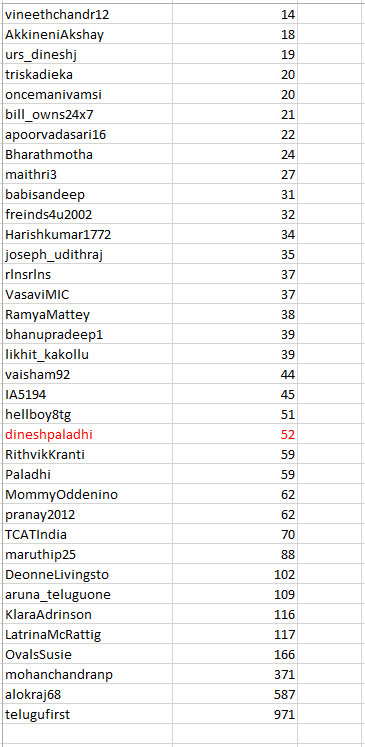
\includegraphics[scale=0.9]{followers_with_source_twt.png}
        \caption{Sample list of Twitter Followers and their count with source}
        \label{Sample_t1}
    \end{center}
\end{figure}
\newpage
\subsubsection{Sample list of Twitter Followers and their count without ``dineshpaladhi''}
\begin{figure}[ht]    
    \begin{center}
        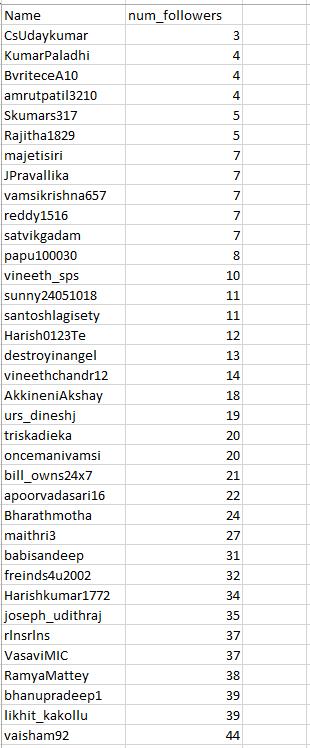
\includegraphics[scale=0.9]{followers_without_source_twt.png}
        \caption{Sample list of Twitter Followers and their count without source}
        \label{Sample_t2}
    \end{center}
\end{figure}
\newpage
\subsubsection{R code and results for Calculation of Mean,Median and Standard Deviation}
\lstinputlisting[language=R,breaklines = true,frame=single,caption={R code for Mean,Median and Standard Deviation}, label=lst:q2R,captionpos=b,numbers=left,showspaces=false,showstringspaces=false,basicstyle=\footnotesize]{calculations_twit.R}

\subsubsection{R code and results for plotting graph between Twitter followers and their count of followers}
\lstinputlisting[language=R,breaklines = true,frame=single,caption={R code for plotting graph between Twitter followers and their count of followers}, label=2nd:q2R,captionpos=b,numbers=left,showspaces=false,showstringspaces=false,basicstyle=\footnotesize]{graph_twit_followers.R}
\newpage
\subsubsection{Graph showing Twitter followers and their count of followers}
\begin{figure}[ht]    
    \begin{center}
        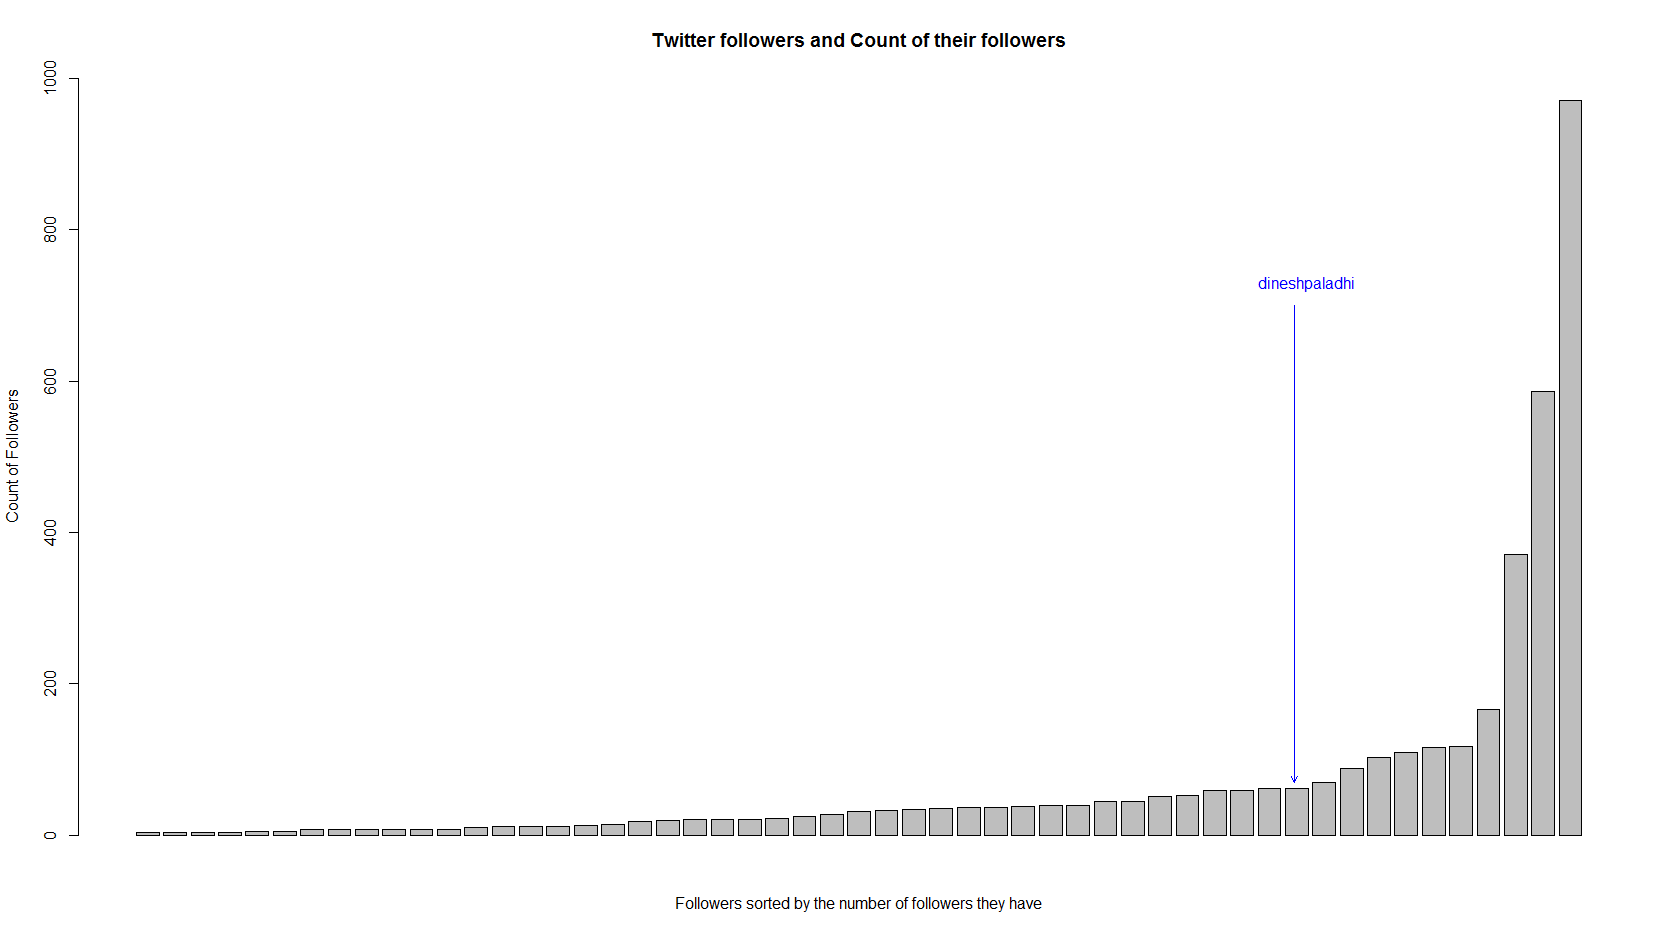
\includegraphics[scale=0.3]{followersgraph.png}
        \caption{Twitter followers and their count of followers}
        \label{graph2}
    \end{center}
\end{figure}
\newpage
